This section outlines the User Interface of the S\&C system, providing an overview of the various pages that form the core of the platform. The design mockups presented in this document focus on interaction dynamics and functionality rather than the final visual aesthetics, acknowledging that graphical elements may undergo adjustments during the testing and refinement phases. While the desktop browser version is emphasized due to its alignment with the platform's primary objective of connecting students and companies, equivalent pages will be designed and optimized for the mobile version to ensure a seamless and responsive user experience across devices.

As highlighted in the RASD, these design mockups serve as an initial representation of the interface and are subject to iterative enhancements based on testing outcomes and user feedback, ensuring that the system meets the expectations of its target audience while maintaining usability and efficiency.


\section{Overview}

\begin{figure}[H]
    \begin{center}
        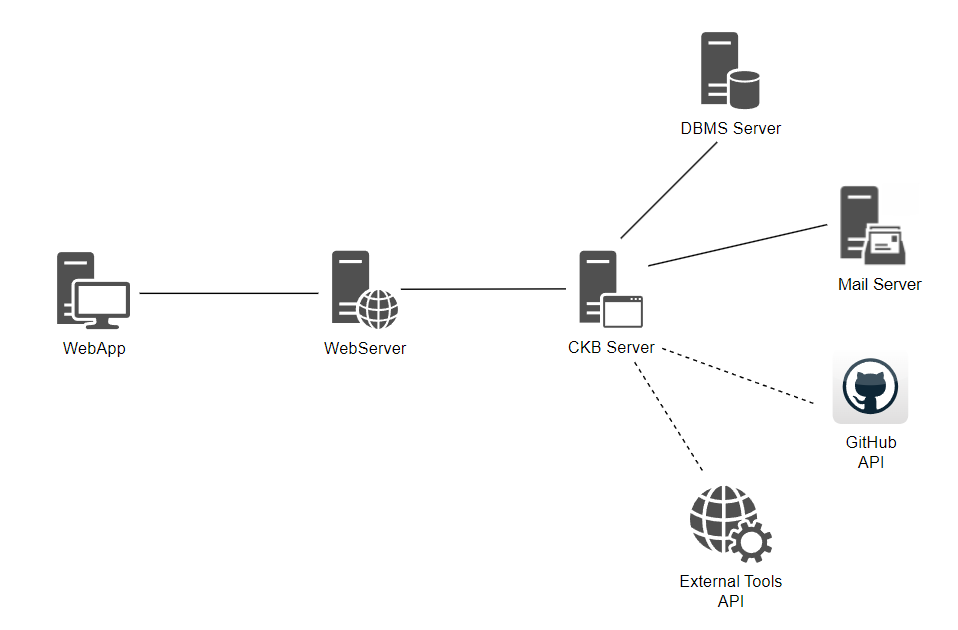
\includegraphics[width=0.8\linewidth]{Interfaces_UI/Overview.png}
        \caption{User Interface Overview.}
        \label{fig:user_interface_overview}%
    \end{center}
\end{figure}

The provided diagram presents a comprehensive overview of the S\&C system’s pages, illustrating their interconnections and the primary pathways for user navigation. Each page serves a specific purpose in enabling seamless interaction between students and companies. Detailed descriptions of each page are provided in the following sections, with the exception of the landing page, which is implicit as it primarily serves as an introduction to the platform and provides access to the login and registration pages.


\section{Header}

\begin{figure}[H]
    \begin{center}
        
\includegraphics[width=1\linewidth]{Interfaces_UI/Header.png}
        \caption{Header.}
        \label{fig:header}%
    \end{center}
\end{figure}

Across all pages in the S\&C system, a uniform header ensures a consistent and user-friendly experience. The header prominently displays the platform name, a notification icon to keep users updated, a menu icon for easy navigation, and the user’s name or identifier. These elements provide quick access to essential features, enhancing usability across the platform.

In cases where the user is a company or a university, the header undergoes slight modifications to better cater to their role. For instance, instead of the user's name, the company or institution’s name is displayed, reflecting their organizational identity. Additionally, the menu options adapt to include functionalities specific to these users, such as "Recommended Students" or "Create Tasks." Despite these changes, the cohesive design of the header remains consistent, ensuring familiarity and accessibility for all users.
 

\newpage

\section{User Interfaces}
\newcounter{ui}
\setcounter{ui}{1}
\newcommand{\cui}{\theui\stepcounter{ui}}

\subsection*{UI\cui . Login and Registration Pages}

\begin{figure}[H]
    \begin{center}
        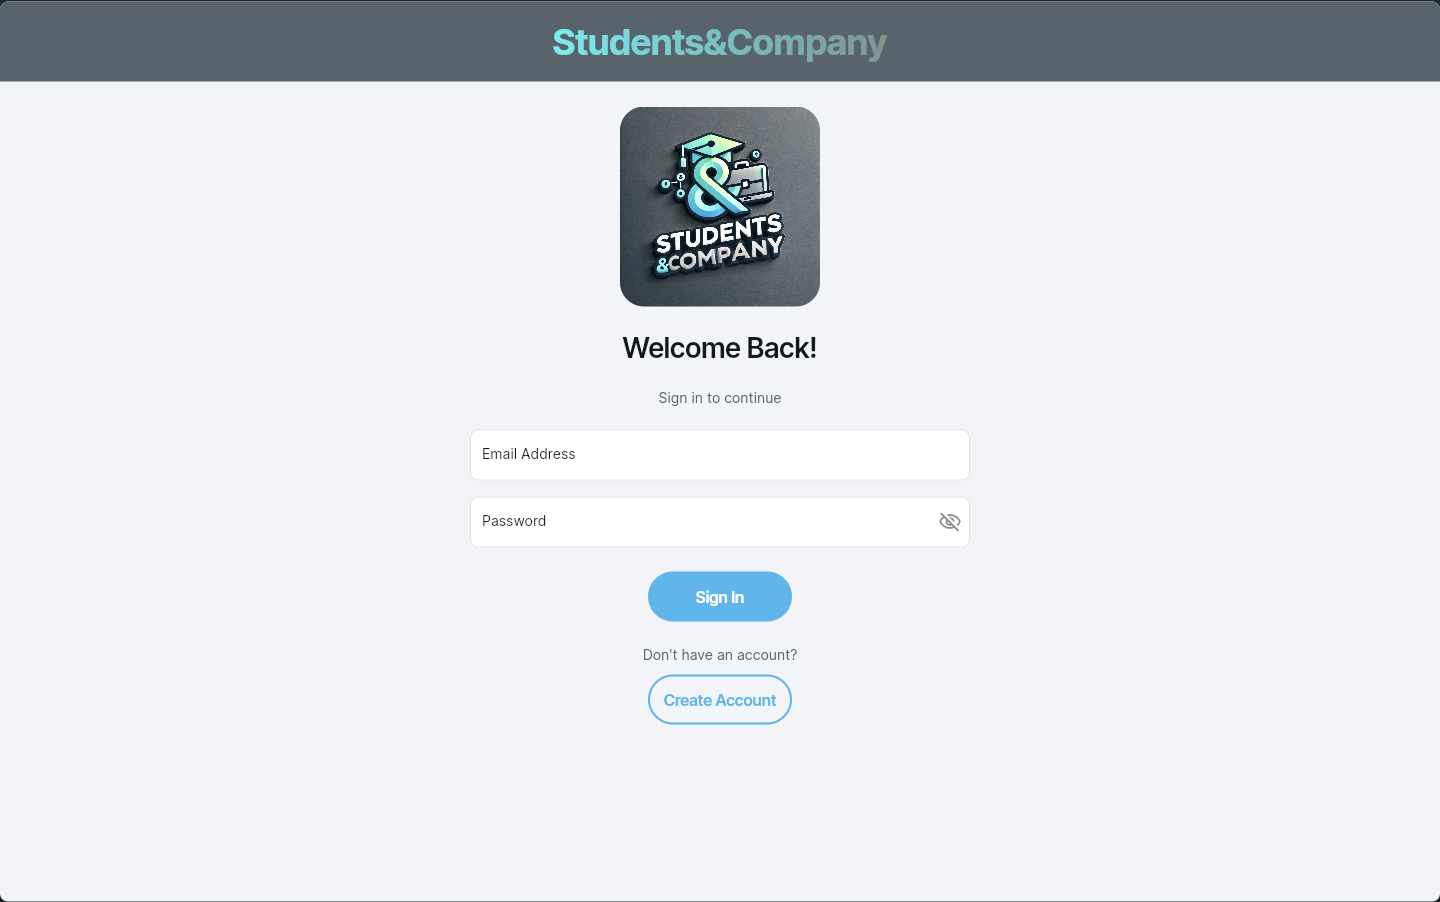
\includegraphics[width=0.7\linewidth]{Interfaces_UI/LoginPage.png}
        \caption{Login Page.}
        \label{fig:login_page}%
    \end{center}

    \begin{center}
        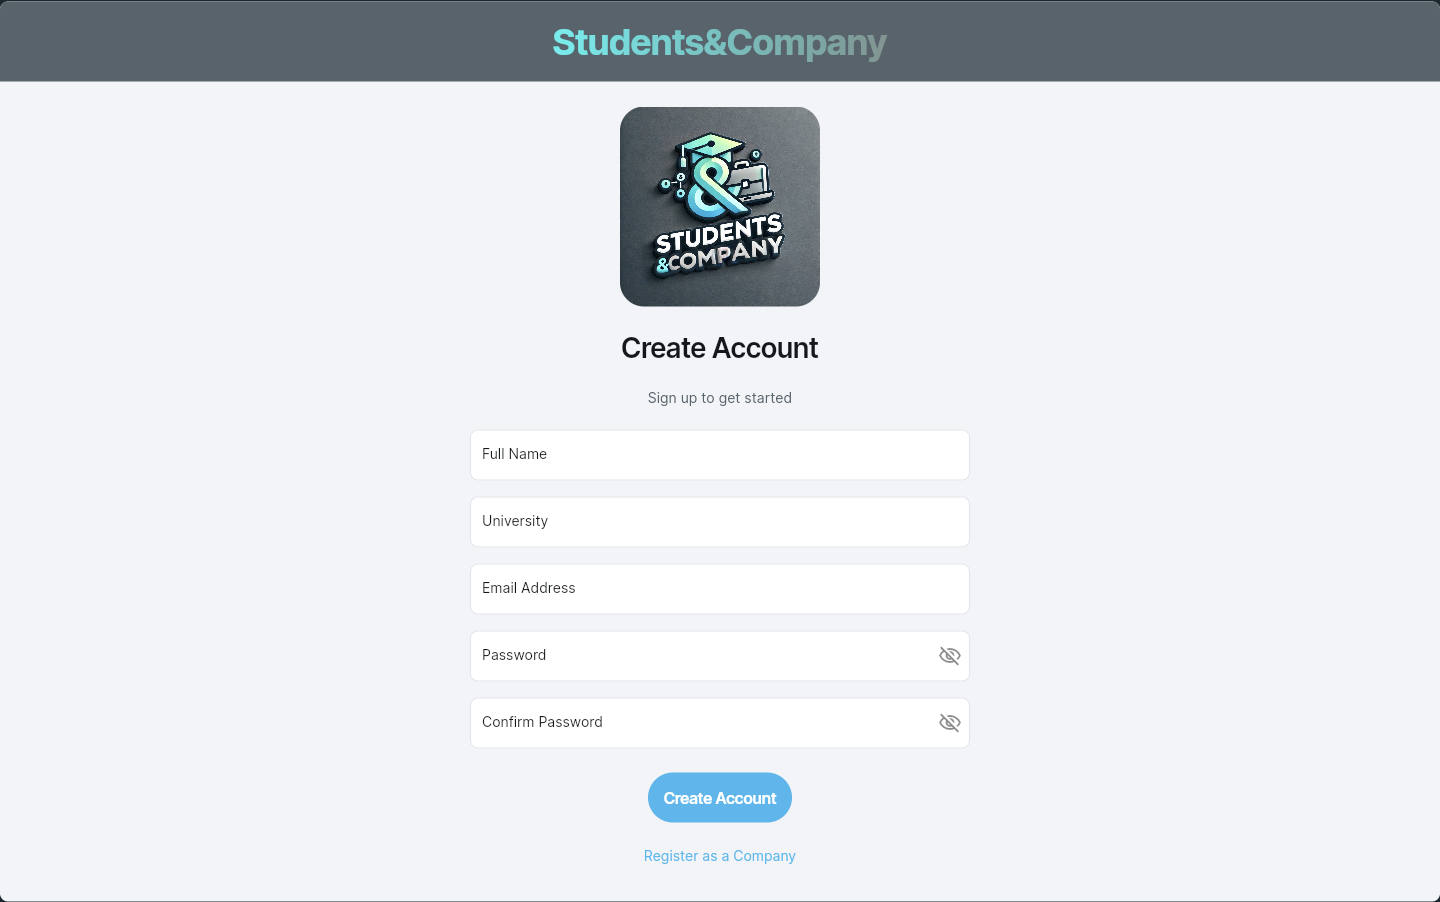
\includegraphics[width=0.7\linewidth]{Interfaces_UI/RegistrationPage.png}
        \caption{Registration Page.}
        \label{fig:registration_page}%
    \end{center}
\end{figure}

The "Login" and "Registration" pages are simple form pages that allow user to register and sign in.  For the Login page, either if the User is a ST or CP or UV, they just need to enter their credentials to login. The registration's steps are a bit different between them, for STs they need to specify their Full name, email, password and the the university they belong to; for both CPs and UVs, they need to specify some other aspects to make sure that not everyone can register as CP or UV.

\subsection*{UI\cui . ST Homepage}

\begin{figure}[H]
    \begin{center}
        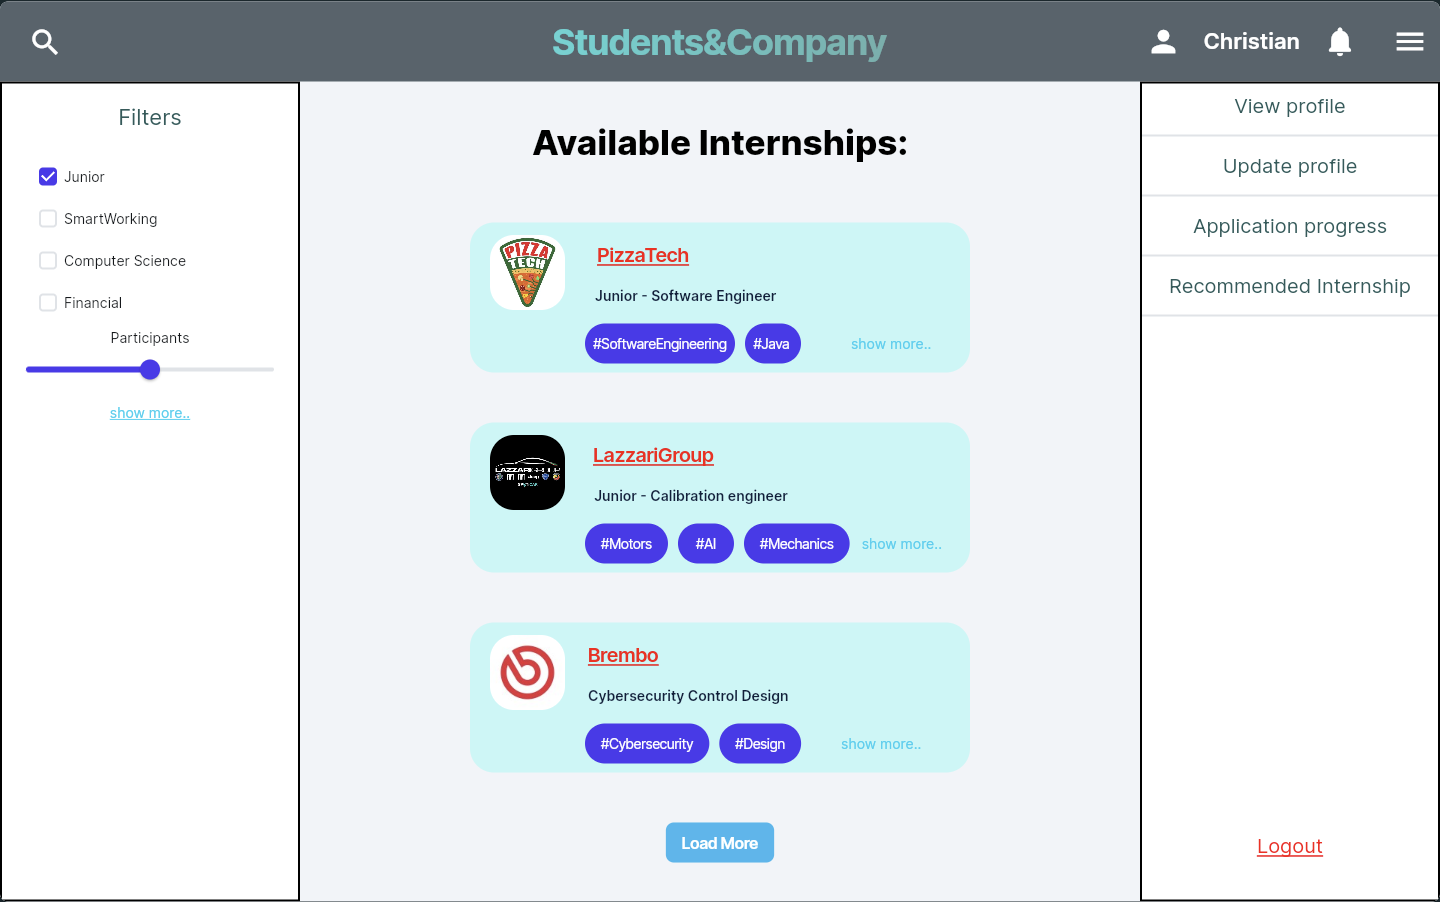
\includegraphics[width=0.7\linewidth]{Interfaces_UI/STHomePage.png}
        \caption{ST Homepage.}
        \label{fig:st_homepage}%
    \end{center}
\end{figure}

From the Login Page, the ST will be redirected to the Student Homepage, which is composed by a scrollable feed of internships in the center. On the left side ST can apply filters for a better search of internships, also with the possibility of a keyword search by writing on the lens at the top. On the right there is a drop-down menu that allows ST to view their profile, update it in the case they have not done it yet, the application progress page that will be explained later, and the possibility to Logout.

\subsection*{UI\cui . Update Profile Page}

\begin{figure}[H]
    \begin{center}
        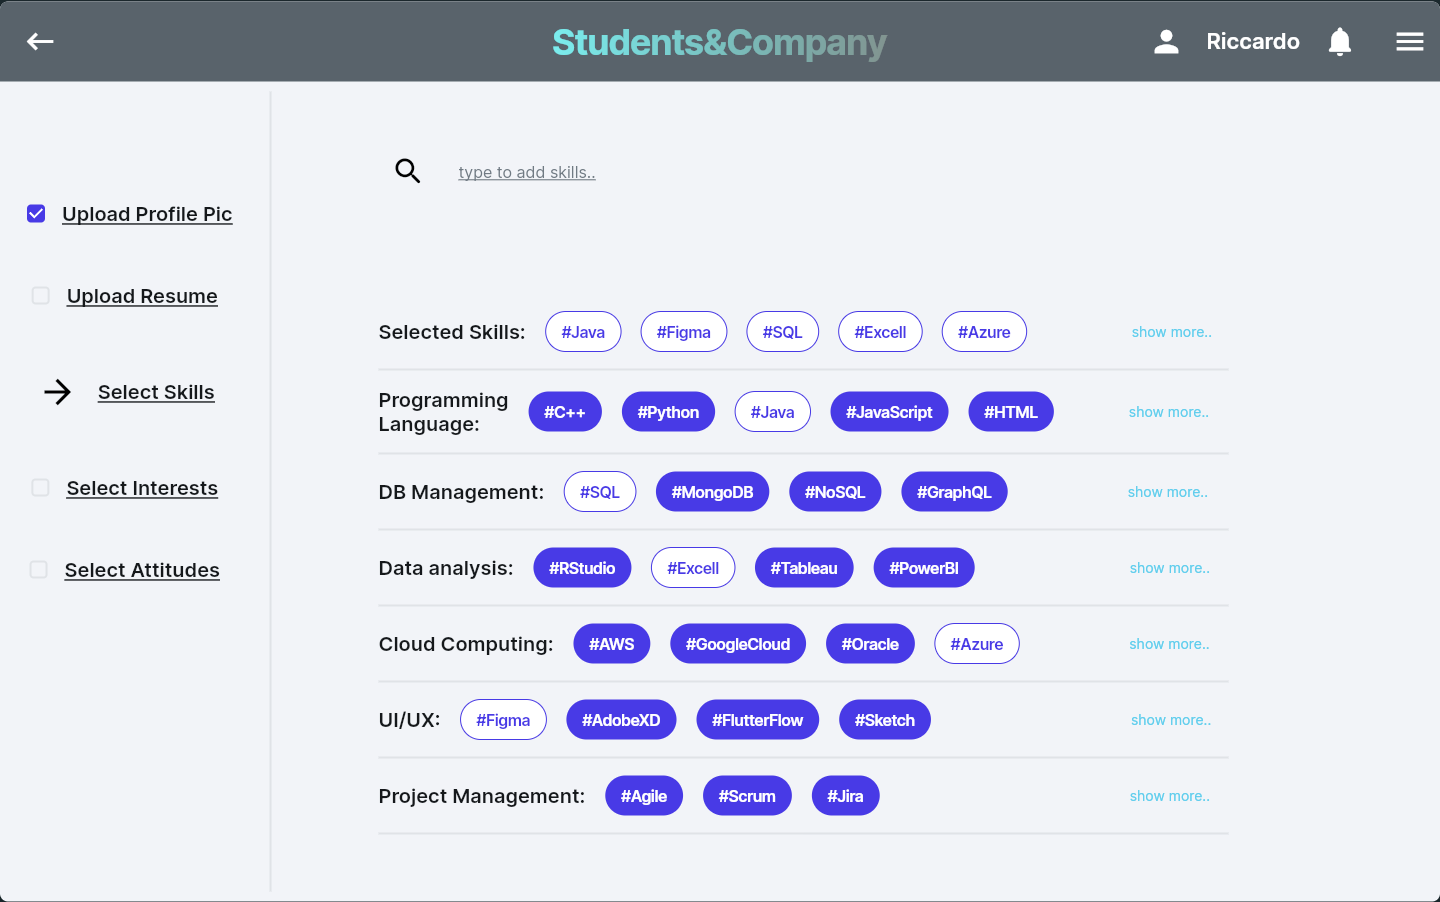
\includegraphics[width=0.7\linewidth]{Interfaces_UI/UpdateProfilePage.png}
        \caption{Update Profile Page.}
        \label{fig:update_profile_page}%
    \end{center}
\end{figure}

The "Update Profile" form page is where the STs can enrich their profile overview by setting some pre-defined parameters that best describe them. This process starts with uploading a profile picture, a resume, select the individual skills, interests and attitude, but anyone can skip any of the steps, knowing that poor profiles are less likely to be matched with the right internship.

\subsection*{UI\cui . CP Homepage}

\begin{figure}[H]
    \begin{center}
        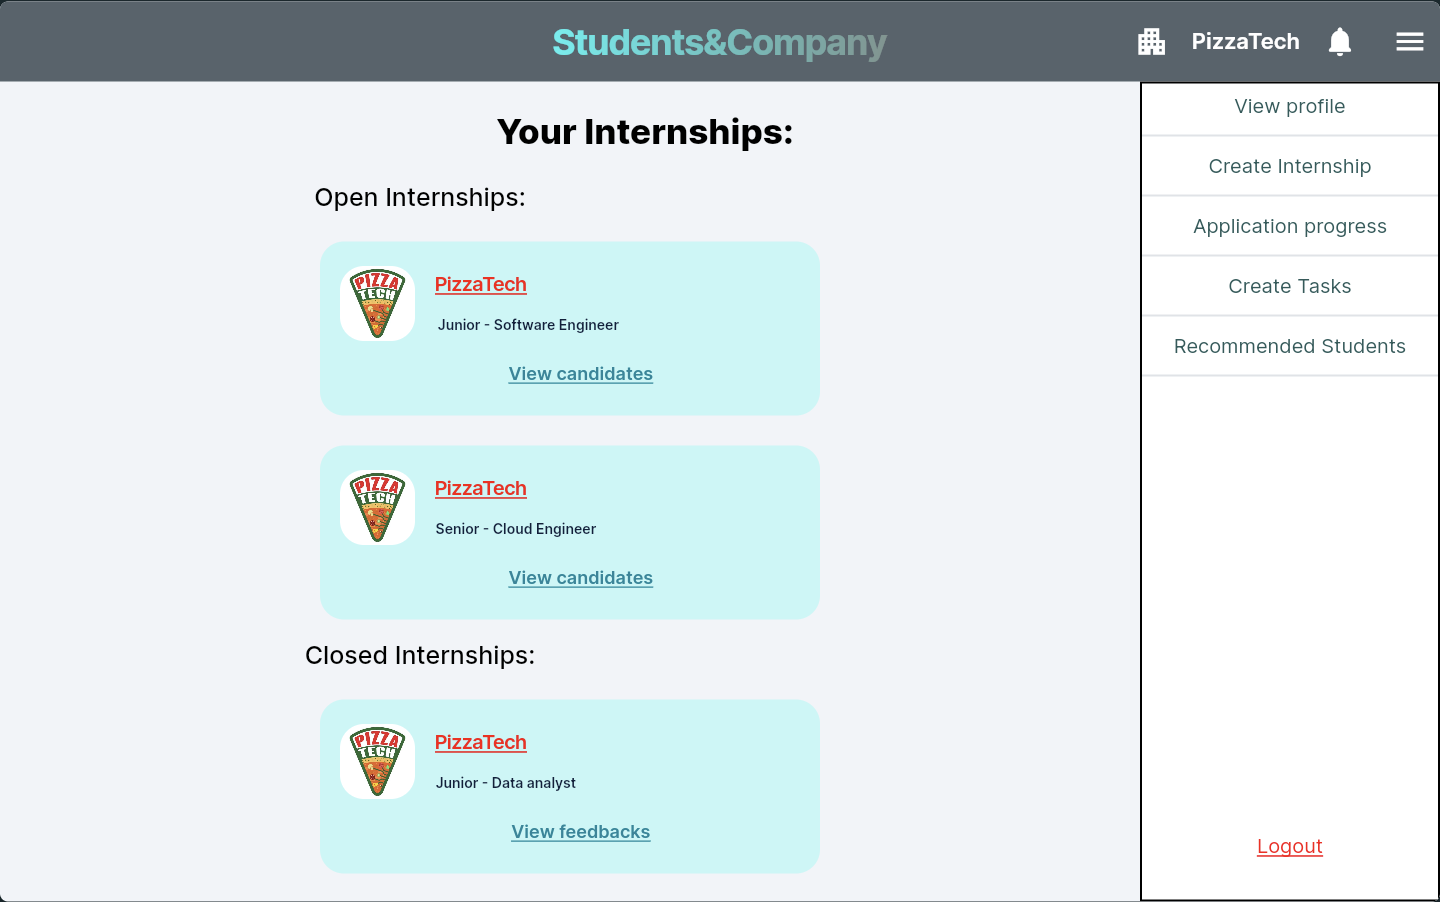
\includegraphics[width=0.7\linewidth]{Interfaces_UI/CPHomePage.png}
        \caption{CP Homepage.}
        \label{fig:company_homepage}%
    \end{center}
\end{figure}

From the Login Page, the CP will be redirected to the Company Homepage, which is composed by the published internship by them. Clicking on top of an internship redirect to the View Internship page, which provides an overview of everything the CP needs to know.

\subsection*{UI\cui . Create Internship Page}

\begin{figure}[H]
    \begin{center}
        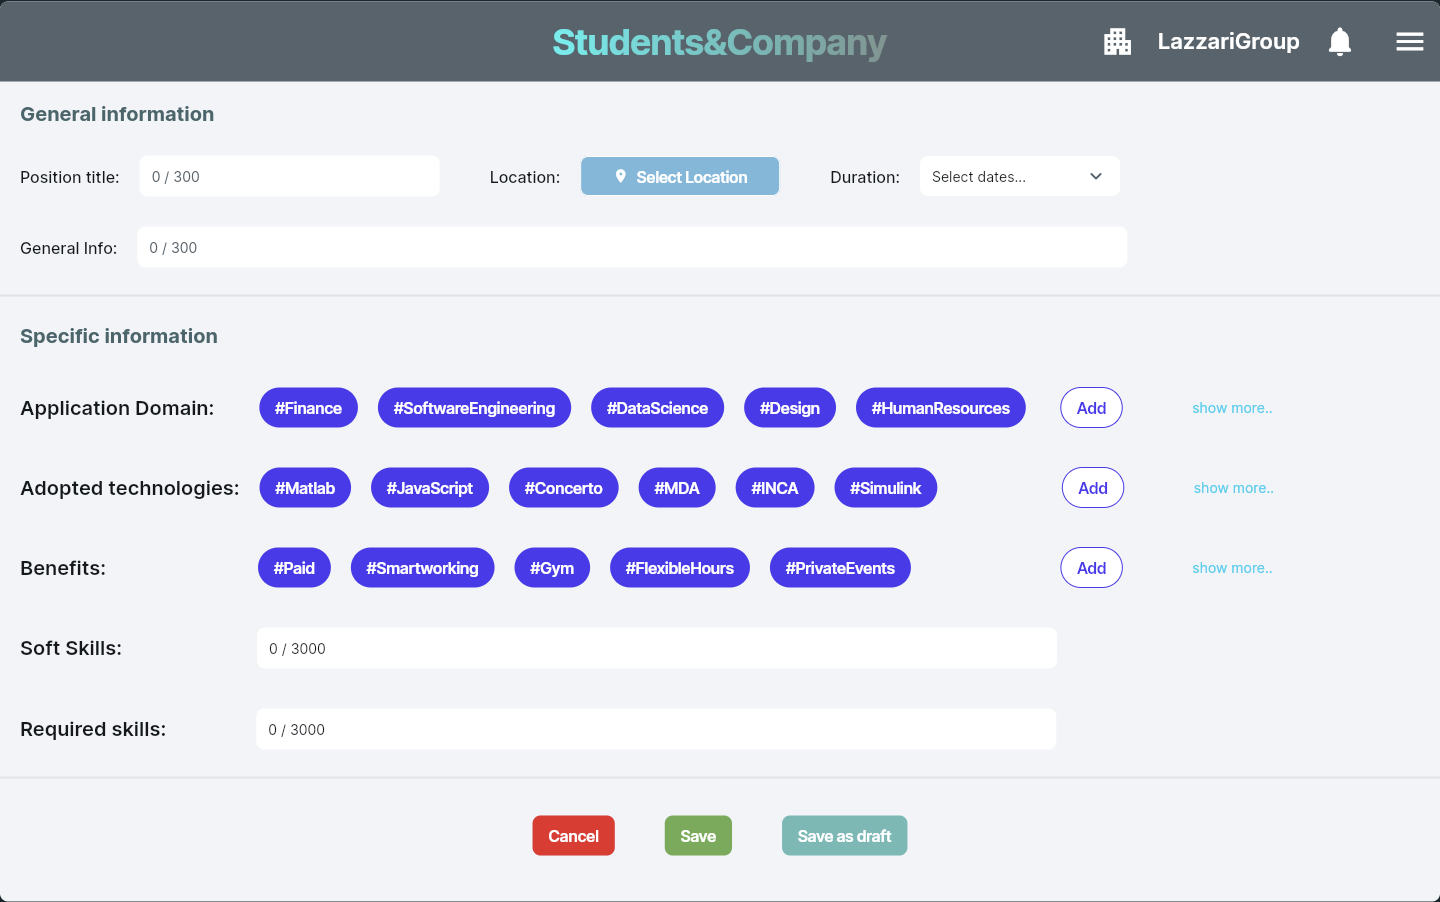
\includegraphics[width=0.7\linewidth]{Interfaces_UI/CreateInternshipPage.png}
        \caption{Create Internship Page.}
        \label{fig:create_internship_page}%
    \end{center}   
\end{figure}

In the "Create Internship" page, the CP can start to create a new announcement for an internship, starting by filling the General information forms, which include the position title, location, duration and some other general info.
After that, the CP can start filling in the specific information forms by selecting some of the predefined tags that could be inherent to the internship they're proposing. At any moment the CP can cancel, pause or publish this process by clicking on the "Cancel", "Save as Draft" or "Publish" buttons at the bottom of the page.

\subsection*{UI\cui . View Profile Page}

\begin{figure}[H]
    \begin{center}
        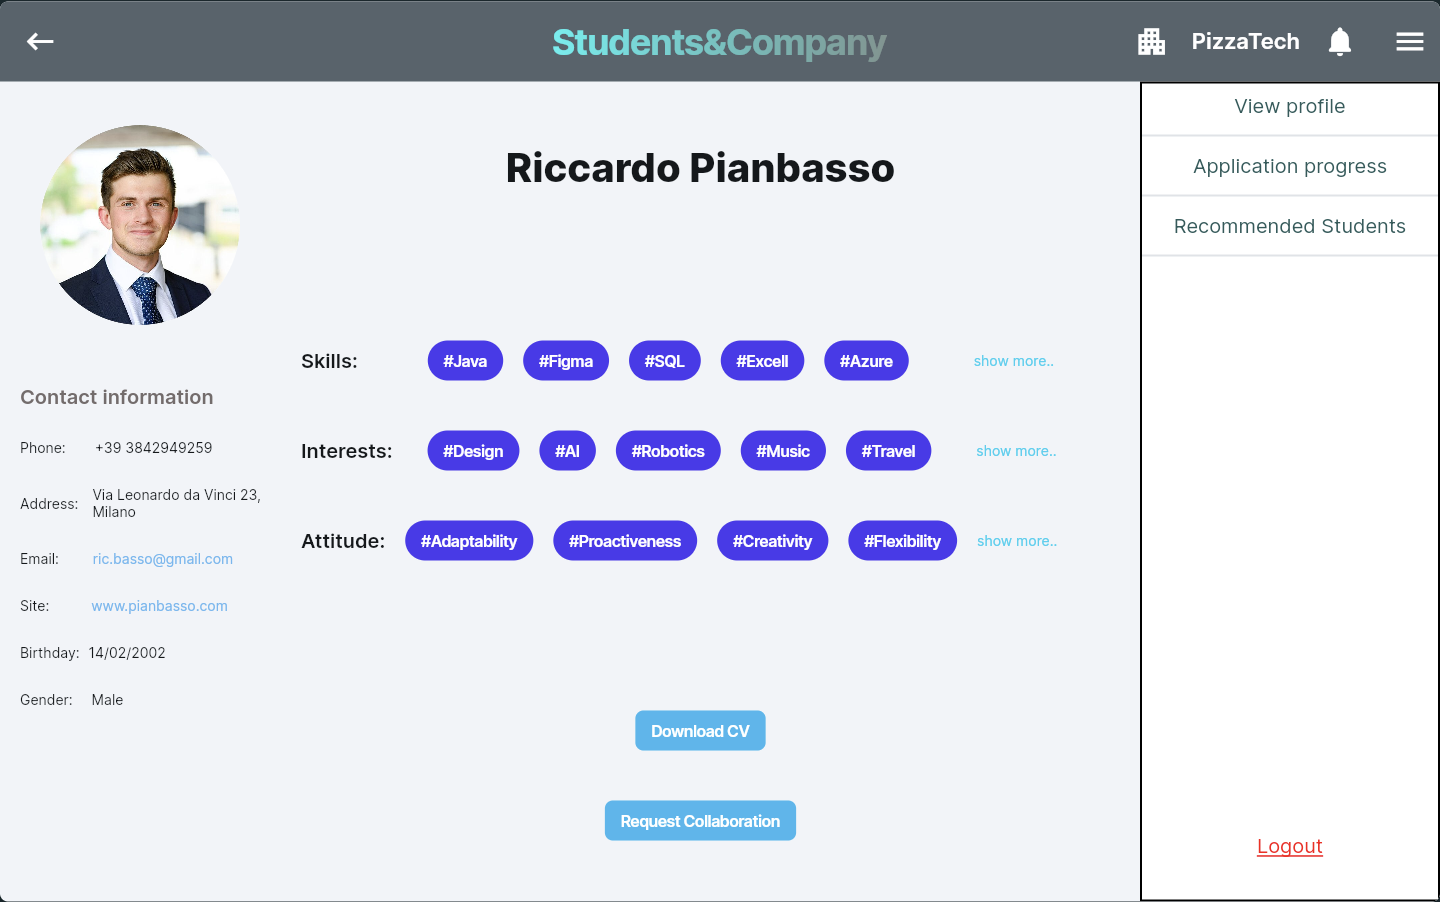
\includegraphics[width=0.7\linewidth]{Interfaces_UI/ViewProfilePage.png}
        \caption{View Profile Page.}
        \label{fig:view_profile_page}%
    \end{center}
\end{figure}

The "View Profile" page provides an overview of the student, and based on the User that is visualizing this page, some functionality may appear. In this case the company PizzaTech has received a matching notification for this student, and now has the possibility to contact him by clicking on the "Request Collaboration" button.

\subsection*{UI\cui . View Internship Page}

\begin{figure}[H]
    \begin{center}
        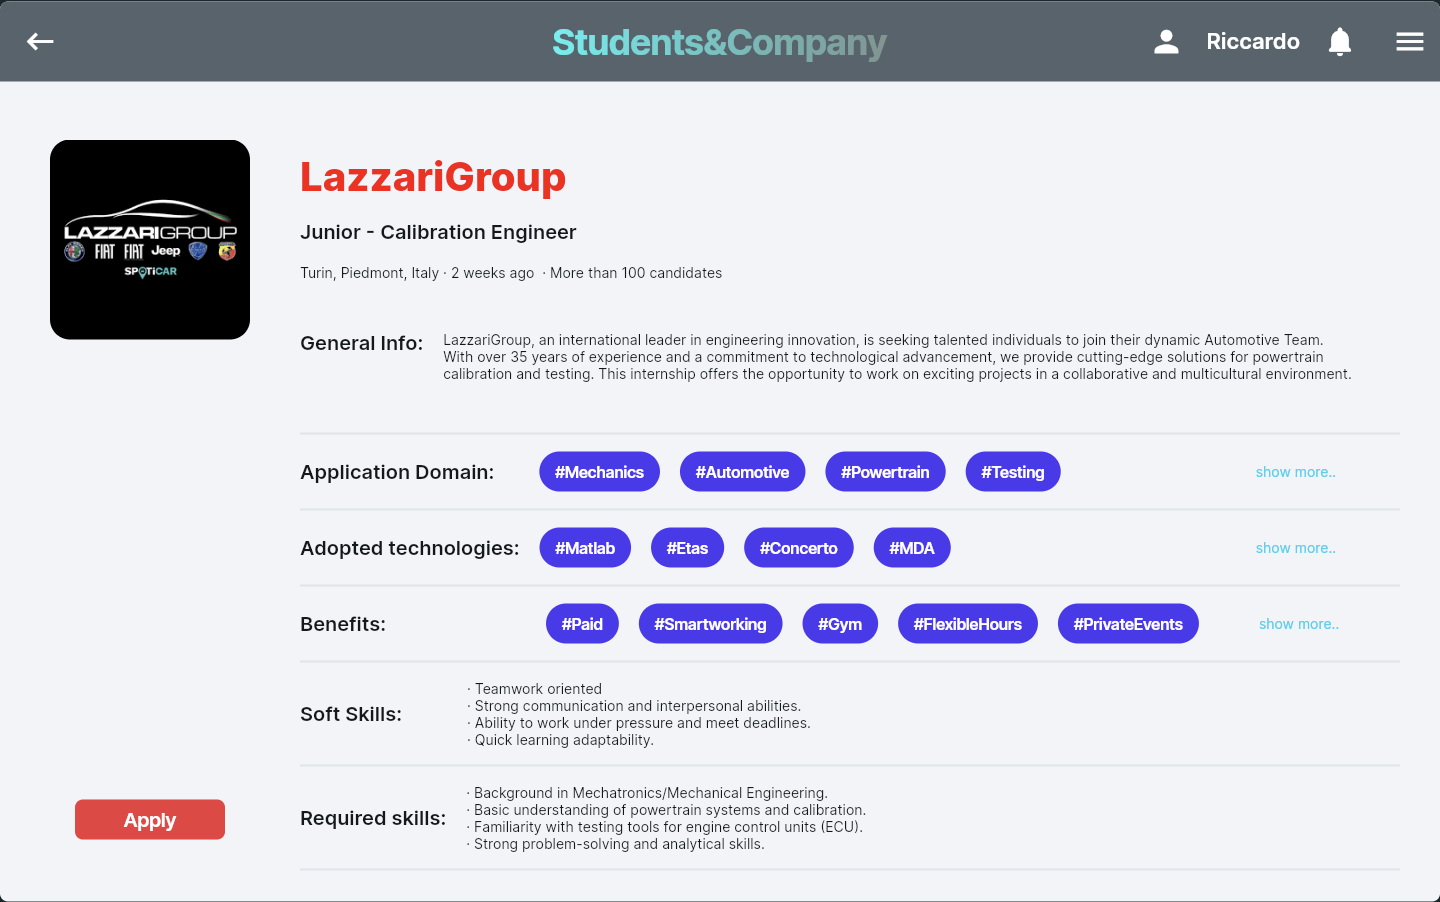
\includegraphics[width=0.7\linewidth]{Interfaces_UI/ViewInternshipPage.png}
        \caption{View Internship Page.}
        \label{fig:view_internship_page}%
    \end{center}
\end{figure}

The "View Internship" page displays all the general and specific information of an internship. Depending on the User who visualizes the page, some changes may appear, as in this case is present the "Apply" button is present, which appears when a ST views this page. In case it is the publishing company that visualizes this page, it can also modify the parameters and the status of the internship.

\subsection*{UI\cui . Application Progress Page}

\begin{figure}[H]
    \begin{center}
        \includegraphics[width=0.7\linewidth]{Interfaces_UI/applicationProgressPage.png}
        \caption{Application Progress Page.}
        \label{fig:application_progress_page}%
    \end{center}   
\end{figure}

The "Application Progress" page allows both Students and Companies to track the status of a specific internship for a student. For a Student, this page provides a clear visualization of the progress of their internship journey, categorized into four distinct phases:

\begin{itemize}
    \item \textbf{Open}: This status represents internships that are still in the initial phase, where applications have been submitted but the selection process has not yet begun.
    \item \textbf{Selection}: In this phase, the company evaluates candidates by assigning tasks or conducting interviews to determine the most suitable applicants.
    \item \textbf{Ongoing}: This is the active phase of the internship, where the student is already working with the company.
    \item \textbf{Closed}: The final phase, marking the completion of the internship. At this stage, students can provide feedback regarding their experience.
\end{itemize}
This page provides an intuitive and structured way for users to understand the progress of each application at a glance.

\subsection*{UI\cui . University HomePage}

\begin{figure}[H]
    \begin{center}
        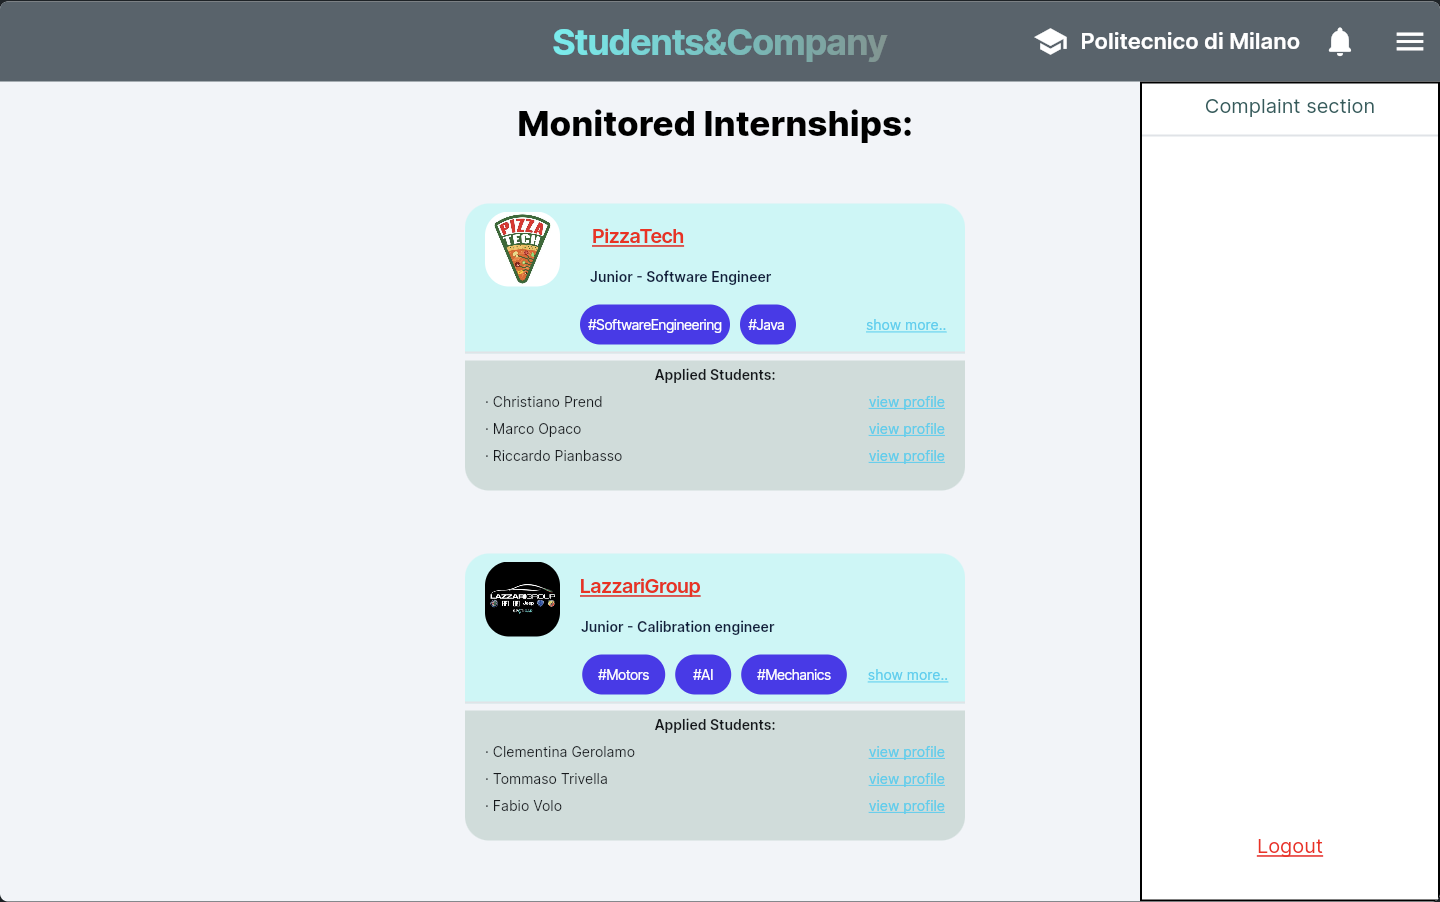
\includegraphics[width=0.7\linewidth]{Interfaces_UI/UVHomePage.png}
        \caption{University Homepage.}
        \label{fig:university_homepage}%
    \end{center}   
\end{figure}

From the Login Page, the UV will be redirected to the University Homepage, where the status of all student's internship can be monitored. After clicking on a view profile for a specific student, the UV can reach the Application Progress page through the View Profile Page. Here it can view the full journey between the Student and it's internship. Also, when a complaint is made, a notification will be received through the notification icon in the header, or the UV can check if there are any complaints on the Manage Complaint Page by clicking on the button placed in the right-side menu. 

\subsection*{UI\cui . Manage Complaints Page}

\begin{figure}[H]
    \begin{center}
        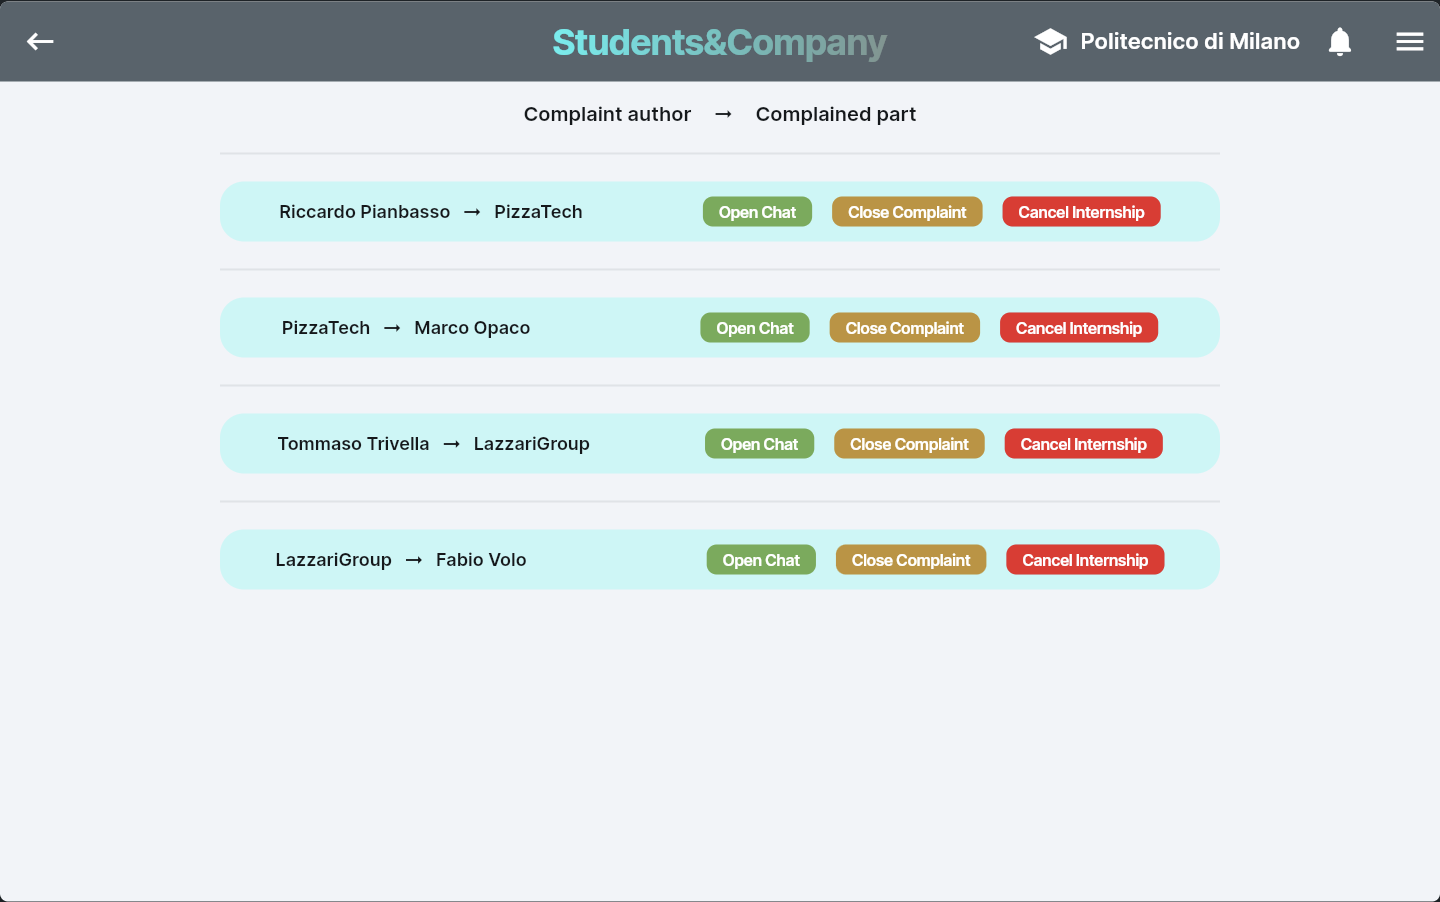
\includegraphics[width=0.7\linewidth]{Interfaces_UI/ManageComplaintsPage.png}
        \caption{Manage Complaints Page.}
        \label{fig:manage_complaints_page}%
    \end{center}   
\end{figure}

From the University Homepage, the UV can reach this Manage Complaints Page, where all the filed complaints are listed there. When a new complaints is made, the UV can ask the complaint author to open a chat to have a better understanding on the situation. After that, the company can decide whether to Mark the complaint as solved or Close the internship.





